% Chaper background Continued .. 
\section{Recommender System}
A recommender system is an Information Filtering (IF) system that provides or suggests relevant items to user based on the user profile and preferences. Basic idea of general recommender model is given in : \autoref{fig:recommender_model} \\

\begin{figure}[H]
	\centering
	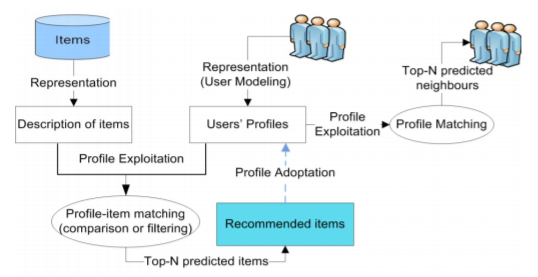
\includegraphics[width=0.7\linewidth]{recommender_model}
	\caption{General Recommender Model \cite{3}}
	\label{fig:recommender_model}
\end{figure}

\noindent Traditionally there are two basic models of recommender systems. \begin{itemize} \item Content based filtering \item Collaborative filtering \end{itemize}


\pagebreak

\subsection{Content Based Filtering}
In Content based method algorithm, user preference is considered based on item description. The rating and buying behavior of users are combined with content information available in the items. The main aim of content based filtering is to create profile for each item and each user to find similar items the user is looking for \cite{6}.
\\

\begin{figure}[H]
	\centering
	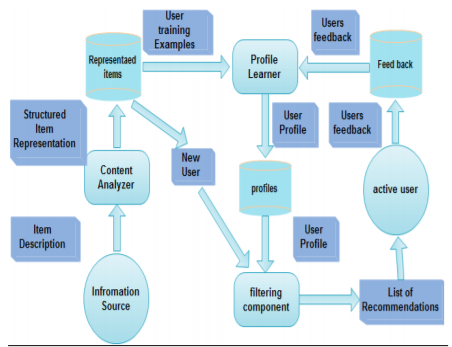
\includegraphics[width=0.7\linewidth]{contentbased_architecture}
	\caption{Content Based filtering Architecture \cite{5}}
	\label{fig:contentbased_architecture}
\end{figure}

\noindent In this algorithm each user's information can be stored in vector form which contains past behavior of the user. This vector is known as profile vector or user profile. All the information about item is stored in item vector / item profile which contains all the details about item specific attributes. Based on similarity score between user profile and item profile most relevant items are recommended to user. 
\\
Advantages of content-based recommenders are – 
\\
Content-based recommender systems are heavily reliable on the contents of the items that have been rated by the user. So, while making recommendations, this approach would consider user’s taste and accordingly recommend an item that matches user’s preferences. Generally, most popular items dominate less popular items. But this approach will not miss less popular item if it matches the user’s unique taste \cite{6}.
\\
Disadvantages of content-based recommenders
\\
User profiles are generated based on rated items. But for any new user who has not rated any items yet, user profile will be empty. In that case, recommending perfect item that matches to user’s taste is difficult as system does not have user taste information. This problem is known as cold start. Also, to understand each items feature, system needs to examine content of every item. Therefore if number of items rises quickly, performance of the system decreases \cite{6}.  
\\

\subsection{Collaborative Filtering}
Collaborative filtering uses other users’ behavior in the system to predict and recommend items. It depends on user’s contribution such as ratings, reviews which considered as filter for user preference information. The fundamental idea of collaborative filtering is, it selects other users opinions and aggregate in such way that it provides prediction for active user based on his preferences \cite{7}. 
\\The main source of input for this algorithm is in the form of matrix of collected user-item ratings. Based on this input it provides recommendations as an output. The first step of output is to predict ratings for items that user may like. Second step is to recommend a list of top rated items as top-N items.
\\

\begin{figure}[H]
	\centering
	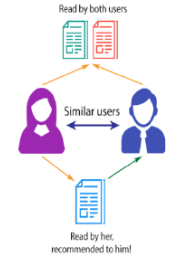
\includegraphics[width=0.7\linewidth]{collaborative_filtering}
	\caption{Collaborative Filtering \cite{8}}
	\label{fig:collaborative_filtering}
\end{figure}


Collaborative Filtering is broadly divided into 2 categories \cite{11}. 
\\
$1.$ Memory-based CF
\\
$2.$ Model-based CF
\\
\subsubsection{A. Memory-Based (user based)}
A memory-based collaborative filtering approach predicts item ratings based on ratings given by different users for an item. There are primary two forms of memory-based collaborative filtering.
\paragraph{i. User-User CF:} 

Similarity between users is calculated based on how similarly they rate several items. It finds other users whose ratings are similar to active user and use their ratings on other items to predict what active user may like. Thus it recommends items to the users that are most preferred by similar users.
\\
Consider example of user and ratings given by users to different recipes. This algorithm will find similarity between each user based on the ratings they have given to the recipes in the past. The prediction of a recipe for a user u is calculated by computing weighted sum of the user ratings given by other users to recipe i.
The prediction for recipe I is given as below:
\\
\begin{equation}
P_{u,v} = \frac { \sum_v(r_{v,i} * S_{u,v})}{\sum_v S_{u,v}}
\end{equation}
\\
Where, 
\\
\noindent
$P_{u,i} = $ \text{prediction of recipe } $i$ 
\\
$R_{v,i} = $ \text{rating given by user} $v$ \text{ to recipe } $i$ 
\\
$S_{u,v} = $\text{similarity between users.} 
\\

\noindent To predict the ratings for other user we need to calculate similarity score. The similarity between users can be calculated with the help of several methods described in the section of \nameref{similarity_methods}. Prior to that we need to find items rated by both users and its rating. Based on that rating, if we opt to calculate similarities with the Pearson correlation then we will get correlation score between users. Higher correlation implied higher similarity. Recommendations are made based on these prediction values. 
\\
This algorithm is quite expensive in terms of time as it involves calculating similarity score between each user and from that score calculating predictions. 
\\
\noindent \paragraph{ii. Item-Item CF:}

Item-Item CF filtering are introduced to solve challenges in User-User CF. As we seen in user user CF may become so expensive if we have large number of users. If we have huge number of users that items then it is ideal to adopt item-based CF.
\\
\\
This algorithm calculates the similarity between items instead of users. It considers ratings of active user to make predictions for item $i$, as $i$ will be similar to the items rated in the past by active user. Therefore, user may prefer to use his own ratings than using some other users' ratings. It helps in maintaining user preferences and choice. The similarity between item can be calculated with any formula from section (add number) cosine similarity, Pearson
correlation,Jacquard or Eucidean's distance formula.
\\
The rating prediction for item-item collaborative filtering is calculated with below equation:
\begin{equation}
P_{u,i} = \frac { \sum_N(S_{i,N} * R_{u,N})}{\sum_N (\vert S_{i,N} \vert)}
\end{equation}
\\
Where, 
\\
\noindent
$P_{u,i} = $ \text{prediction of item $i$ for user } $u$ 
\\
$R_{u,N} = $ \text{rating given by user } $u$ \text{ on item } $N$ 
\\
$S_{i,N} = $\text{similarity between item $i$ and $N$.} 
\\
\\
Memory based collaborative filtering can be useful in any area where we don't need to select many features. At the same time it suffers from dome drawbacks \cite{10}.
\\
\\
\textbf{Sparsity:}
\\
Many large systems that uses recommender systems to recommend their products has huge number of products in their database. All products are not rated by users. In that case, ratio of actual number of items to number of rated items is very huge. Because of such huge sparsity accuracy of recommender may result in poor recommendations.
\\
\\
\textbf{Scalability:}
\\
Nearest neighbor algorithm requires high computations. It grows with number of users and number of items in the system. Any web-based system which has huge number o items and users (example Amazon.com) may suffer from high scalability.

\subsubsection{B. Model-Based (item based):}
In contrary to memory-based collaborative filtering, model-based algorithm take the data that has been already preprocessed where it is cleansed, filtered and transformed and generate learned model to make predictions. This algorithm calculates similarity between users or items by generating a model and analyzing their pattern to predict ratings on unseen items \cite{28,29,30} .
\\
Model-based collaborative filter has several techniques such as Slope one \cite{31}, Matrix Factorization (MF) and Singular Value Decomposition (SVD) \cite{28}. 

%based on SVD, SVD++, Matrix Factorization using gradient descent, Co-clusturing, Slope one approach.
In this section we will see frequently used model-based techniques.
\\

\paragraph{i. Singular Value Decomposition (SVD) }
SVD is a technique of matrix factorization which is used to reduce the number of features in the data set. The matrix factorization is done on the matrix which is generated by the user's feedback in the form of ratings on different items. In SVD, the technique is used to detect latent relationship between users and items. Then it generate a low dimensional representation of original matrix space to calculate neighborhood in the reduced space \cite{32}. The original ratings matrix decomposes by SVD in two matrices in such way that product of decomposed matrices is original rating matrix. The SVD is calculated as shown in \autoref{eq:svd}

\begin{equation}
SVD(M) = U \times S \times V^{T} 
\label{svd}
\end{equation}
\noindent Where,\\
$SVD(M)$ denotes matrix M with dimensions $m \times n$ which are total number of users and items respectively.\\
Dimensions of matrix $U$ will be $m \times m$ \\
Dimensions of matrix $S$ will be $m \times r$ \\
Dimensions of matrix $V$ will be $r \times n$ \\
$U$ and $V$ are called left and right singular vectors. To reduce features of dataset one can keep only k highest values and eliminate lower entries. So, $(r-k)$ columns from $U$ and $(r-k)$ rows from $V^{T}$ are discarded to gnerate $U_{k}$ and $V_{k}^{T}$ matrices. Now $M_{k}$ can be constructed with multiplication of $U_{k}$ and $V_{k}$ together using $S_{k}$. Generated $M_{k}$ will closest rank $k$ matrix to $M$. Mathematically it can be represented as in \autoref{eq:svd1}

\begin{equation}
M_{k} = U_{k} \times S_{k} \times V_{k}^{T} 
\label{svd1}
\end{equation}

\noindent Rating prediction for user $u$ for item $i$ is given in \autoref{eq:svd2} \\

\begin{equation}
r_{ui} = r_{u} + U_{k} \sqrt{S_{k}^{T} (u)} \times \sqrt{S_k} \times V_{k}^{T}
\label{svd2}
\end{equation}

\noindent With SVD we can predict ratings with good accuracy.



